\section{Exploring GAP types}\label{sec:gaptypes} 

\subsection{Brief introduction to GAP types and categories.}\label{gap-types-intro}

%\ednote{MP: I am not sure what I claim below about \Sage is true, it
%  also irks me a bit that we seem to conflate the idea of a type system with
%  the idea of organising mathematical hierarchies. Of course in \GAP
%  system this is intentional, in \Sage, I don't know. In my head \Sage
%  uses whatever python uses as the type system (duck typing?) and then intro-
%  duces a category system on top. We should agree on a level of description
%  that fits.}

While the \Sage type system is object-oriented, the \GAP type
system puts more of an emphasis on \emph{operations} on and between objects.

Breuer and Linton describe the \GAP type system in \cite{breuer-linton}, and
the \GAP documentation \cite{GAP4} also contains an extensive technical
description of the \GAP type system.

A type in \GAP is a pair consisting of a \emph{family} and a \emph{filter}.

Families partition the space of objects in \GAP, so every object lies in exactly one family.

A filter is a set of \emph{elementary filters}, and hence filters form a hierarchy on
objects by the subset relation on filters.
We say that an object is \emph{in a filter $F$} if its type's filter component
contains $F$ as a subset.

\emph{Operations} in \GAP are declared with an arity and for each argument with a
most general filter for which they are applicable. For instance there is an operation
for forming the direct product of two groups.
The programmer can install \emph{methods} for an operation which can carry strictly
more specific filters for the inputs.

At runtime \GAP through a very sophisticated mechanism called \emph{method selection} will
select the most appropriate method for the given arguments to an operation and execute it.

\emph{Categories} are filters that model mathematically similar objets. In terms of
algebraic structures we can think of a category as the signature of the structure.
For instance there are categories called \texttt{IsMagma}, \texttt{IsMagmaWithOne}, and
\texttt{IsMagmaWithInverses}, which we can think of as objects having signature $\{ * \}$,
$\{*,1\}$, and $\{*,^{-1}\}$ respectively. Semigroups, monoids, or groups are not
categories in \GAP.

Once an object is created, the category it is in cannot be altered.

\emph{Representations} are filters that give a way to represent mathematical
objects in different ways. One of the examples from the \GAP library are permutations
which can be represented in 2-bytes acting on at most 65536 points, or 4 bytes, acting
on at most $2^{32}-1$ points. Other examples include matrices in sparse or dense
representation, or finite field elements, where particularly matrices with entries in
the field of order 2 allow a very efficient representation.

A \emph{Property} \texttt{P} is realised by two filters \texttt{P} and \texttt{HasP} and an
operation which is also called \texttt{P}.

This models three possible states for a property: Its value can either be known or unknown,
which is reflected by the filter \texttt{HasP}, and if it is known, then the filter \texttt{P}
says whether the property holds or not.
If the value of the property is unknown, but there are methods installed for the operation
\texttt{P}, then \GAP will be attempt to compute the value of \texttt{P} using that method.

Examples of properties in \GAP are \texttt{IsAssociative}
or \texttt{IsCommutative}. A group in \GAP is an object that is in the filter
\texttt{IsMagmaWithInverses} and \texttt{IsAssociative}. An abelian group will additionally
be in the filter \texttt{IsCommutative}.

An \emph{attribute} in \GAP is a value attached to a \GAP object. There is
a filter attached with each attribute that reflects whether the value
of the attribute is known, and an operation which can be invoked to determine
the value of the attribute if it is not known.
\texttt{Size} or \texttt{Centre} are two attributes that are defined for groups.

The values of attributes and properties can be unknown on creation,
can be computed on demand, and their values can then be stored for later
reuse without the need to be recomputed. Note that in particular the knowledge
accumulated in the type of a \GAP object can influence method selection, so for
example attaining the knowledge that a group is nilpotent will allow for more
efficient methods to be run for finding its centre.

\begin{lstlisting}
gap> IsGroup;
<Filter "(IsMagmaWithInverses and IsAssociative)">
gap> IsMagmaWithInverses;
<Category "IsMagmaWithInverses">
gap> IsAssociative;
<Property "IsAssociative">
gap> IsSet;
<Property "IsSSortedList">
gap> IsFinite;
<Property "IsFinite">
gap> IsSet=IsSSortedList;
true
gap> G := Group((1,2), (2,3,4));
Group([ (1,2) ])
gap> HasSize(G);
false
gap> HasIsCommutative(G);
false
gap> Size(G);
24
gap> HasSize(G);
true
\end{lstlisting}

\ednote{TODO (???) Compare and contrast it with the Sage type system}

\subsection{Tentative approaches to exporting GAP types.}\label{gap-types-export}

Encoded in filters, categories, representations, attributes, and properties in \GAP
there is a wealth of mathematical knowledge. \GAP allows some introspection
of this knowledge after the system is loaded.

Having a clear picture of the relations between different objects is 
very helpful to GAP developers, package authors, and users.
For example one might be interested in the attributes or properties that \GAP can
compute for an object, or how it tries to compute them.

During the OpenDreamKit workshop in St~Andrews in January 2016 we developed
tools to more conveniently access mathematical knowledge encoded in \GAP,
such as introspection inside a running \GAP session, export to JSON to import
to MMT, and export as a graph for visualisation and exploration.
\ednote{picture based on \url{https://github.com/OpenDreamKit/OpenDreamKit/issues/165}?}

We will make these tools available as part of the standard \GAP distribution with the next
major release of \GAP, as they will prove useful in the development of the \GAP Jupyter interface
\url{https://github.com/gap-packages/jupyter-gap}, and possibly to do
internal consistency checks of \GAP types.

As a side-effect of the work outlined above, we fixed a number of bugs in the handling of
special categories in \GAP.

The JSON output of the \GAP object system after loading a default set of packages is currently
around 11 Megabytes in size and takes many hours to import into MMT. We did not yet attempt to
load a collection of \GAP packages that would expose even more data.

The graph exported for visualisation has 540 vertices, 759 edges and 8 connected components, if
packages are loaded this increses to 1616 vertices, 2178 edges and 17 connected components.

\centerline{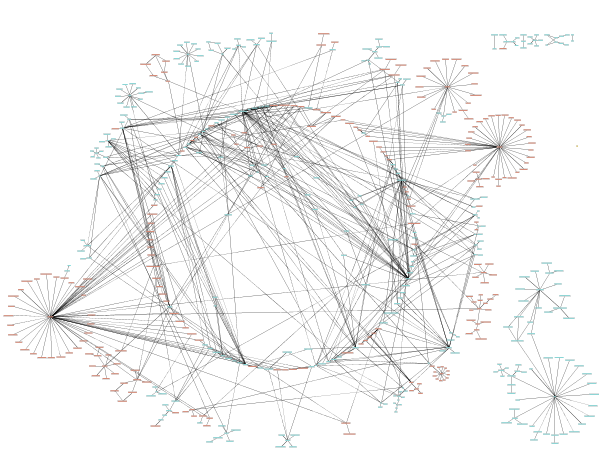
\includegraphics[width=10cm]{gap-graph.png}}

\ednote{NT: Do you have anything to say about the GAP-MMT formalization? 
E.g. hints on potential ways this formalization may be written?}
\ednote{MP: I have some ideas as to how I would write an MMT formalisation, unfortunately I do not
  understand MMT well enough yet to know whether my ideas make any sense. I'll think about this a bit
  more and add my comments then\\
       MP: Also, what exactly are we talking about when we talk about MMT formalisation? The description
  of an export, or how to implement structures exported from MMT in GAP?}

\subsection{An application: consistency checker for the GAP
  documentation.}\label{gap-types}

One of the immediate outcomes of the development of the tools described in the
previous section is the consistency checker for the GAP documentation. 

GAP uses special format for its main manuals. It is called GAPDoc and is 
provided by the GAP package with the same name \cite{gapdoc}. Besides main 
manuals, it is adopted by 97 out of 130 packages currently redistributed 
with GAP. Using GAPDoc, one builds text, PDF and HTML versions of the manual
from a common source given in XML.

GAPDoc defines XML constructions to specify the type of the documented object 
(function, operation, attribute, property, etc.). However, due to the 
limitations of the semi-automated conversion of GAP manuals from the \TeX-based
manuals used in GAP 4.4.12 and earlier, a number of objects had their types
stated incorrectly. 

We developed the consistency checker for the GAP documentation, which extracts
type annotations from the documented GAP objects and compares them with their
actual types. It immediately reported almost 400 inconsistencies out of 3674 
manual entries. In the subsequent cleanup, we by now have eliminated about 
75\% of them. The  consistency checker will appear in the next release of
GAP 4.8.3, and will be available via \texttt{make check-manuals}.
It also performs other useful checks: for example, it produces a list of
manual sections having no examples. Thus, the new tool helps to improve
the quality of GAP documentation, and may be useful for the similar checks
of those GAP packages which use GAPDoc-based manuals.

% \url{https://github.com/gap-system/gap/pull/675}
% \url{https://github.com/gap-system/gap/pull/538}

%%% Local Variables:
%%% mode: latex
%%% TeX-master: "paper"
%%% End:

%  LocalWords:  ednote emph breuer-linton texttt texttt itemize Jupyter formalization
%  LocalWords:  gapdoc gaptypes
